\section{Аналитический раздел}

\subsection{Сущности}
Были выделены следующие сущности

\begin{itemize}

\item Проект

Сущность, определяющая набор данных одного типа и одного типа разметки, относящихся к одной тематике.

\item Пользователь

Сущность, которая содержит информацию о пользователе: администраторе или обычном.
Может иметь привелегии относящиеся к различным проектам.

\item Привелегия (право)

Сущность, которая контролирует возможности пользователей 
размечать данные определенного проекта.

\item Элемент выборки

Сущность, содержащая информацию о конкретном элементе данных, принадлежащих проекту.

\item Метка

Ответ пользователя данный им в процессе разметки для конкретного элемента выборки.

\item Схема проекта
Сущность, содержащая информацию о множестве допустимых значений элементов выборки и меток.

\item Сессия

Сущность, содержащая информацию о подключении пользователя.

\end{itemize}

\subsection{Роли}
Для пользователей приложения выделены следующие роли:

\begin{itemize}
\item Администратор

Имеют возможность создавать проекты, загружать выборку и выгружать метки для созданных ими проектов, предоставлять и лишать
других пользователей привелегий для разметки принадлежащих им проектов, осуществлять разметку проектов к которым имеют привелегии.

\item Обычный пользователь 
Имеют возможность осуществлять разметку данных проектов, в соответствии с привелегиями, предоставленными администраторами. 

\end{itemize}

\begin{figure}
    \caption{Use-Case диаграма}
    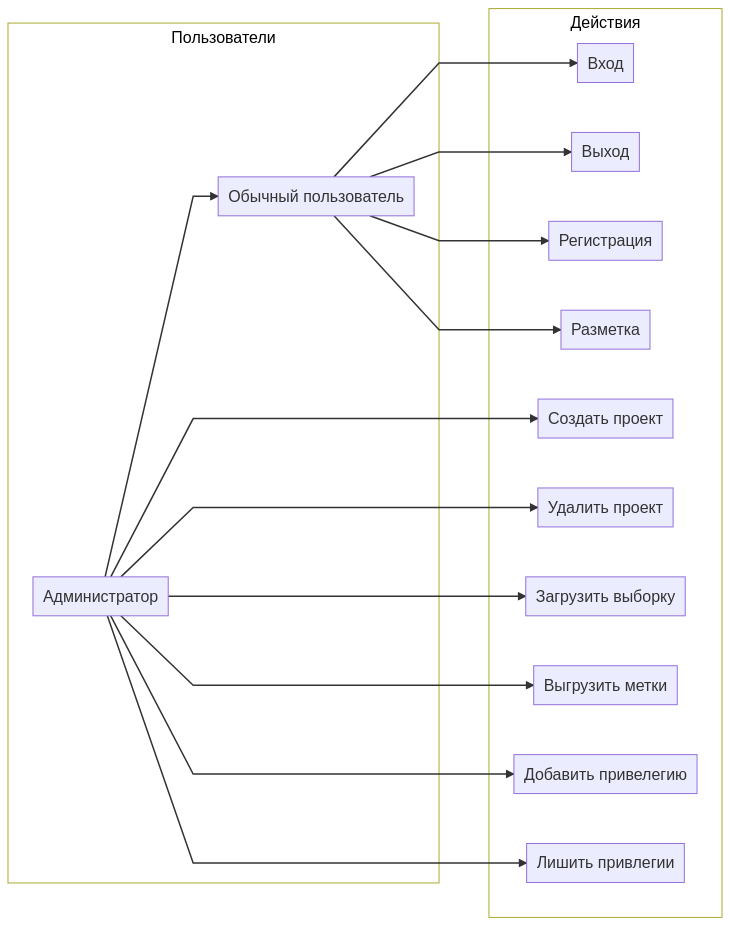
\includegraphics[width=0.9\textwidth]{./use-case.png}
\end{figure}
